\documentclass{article}
\usepackage{arxiv}

\usepackage{hyperref}
\usepackage{url}
\usepackage{amsmath}
\usepackage{mathrsfs}
\usepackage{bm}
\usepackage{amsthm}
\usepackage{amssymb}
\usepackage{array}
\usepackage[dvipsnames]{xcolor}
\usepackage{graphicx} 
\usepackage{booktabs} % for professional tables
\usepackage{makecell} 
\usepackage[figuresright]{rotating}
\usepackage{mathtools}
\usepackage{makecell}
\usepackage{enumitem}
\usepackage{subcaption}
\renewcommand\theadfont{\scriptsize}

% load shortex containing useful packages and shorthand notation
\usepackage[numbers]{natbib}
\bibliographystyle{abbrvnat}
\usepackage[utf8]{inputenc} % allow utf-8 input
\usepackage[T1]{fontenc}    % use 8-bit T1 fonts
\usepackage{url}            % simple URL typesetting
\usepackage{booktabs}       % professional-quality tables

% Latin
\usepackage{xspace}
\newcommand{\eg}{\textit{e.g.}\xspace}
\newcommand{\ie}{\textit{i.e.}\xspace}
\newcommand{\cf}{\textit{cf.}\xspace}
\def\wrt{w.r.t.\xspace}

% useful macros
\def\note#1{\textcolor{blue}{\textbf{Note}: #1}\xspace}
\def\code#1{\colorbox{gray!15}{\small \textcolor{Bittersweet}{\texttt{#1}}}}
\def\todo#1{\textcolor{blue}{\textbf{Todo}: #1}\xspace} 
\def\eqnote#1{\intertext{(\raggedleft #1)}}




% additional macros for highlighting
\usepackage{shortex-light} % needs to be loaded after hyperref
\definecolor{mypurple}{rgb}{0.478, 0.369, 1.0}
\definecolor{myblue}{rgb}{0.2, 0.6, 1.0}
\definecolor{mygreen}{rgb}{0.2, 0.667, 0.2}

%%%%%%%%%%%%%%%%%%%%%%%%%%%%%%%%%%%%%%%%%%%%%%%%%%%%%%%%%%%%%%%%%%%%%%%%%%%%%%%%%%%%%%%%%%%%%%%%%%%%%%%%%%%
\newcommand{\BigO}{\mathcal{O}}


%%%%%%%%%%%%%%%%%%%%%%%%%%%%%%%%%%%%%%%%%%%%%%%%%%%%%%%%%%%%%%%%%%%%%%%%%%%%%%%%%%%%%%%%%%%%%%%%%%%%%%%%%%%
% Fill out paper:
\begin{document}
\title{LLM Notes}

\date{\today}                       
\maketitle
\tableofcontents
\clearpage


\section{Attention}
\subsection{Self Attention}
Given input $\bX \in \reals^{T \times D}$ where $T$ is the sequence length and $D$ is the embedding dimension, we have
\[
\bQ = \bW_Q \bX \in \reals^{T \times d_k} \quad \bK= \bW_K \bX \in \reals^{T \times d_k} \quad \bV = \bW_V \bX \in \reals^{T \times d_v}
\]
\[
\text{Attn}(\bQ, \bK, \bV) = \text{softmax} \left(\frac{\bQ \bK^\top}{\sqrt{d_k}} \right) \bV
\]

\begin{figure}[h]
\centering
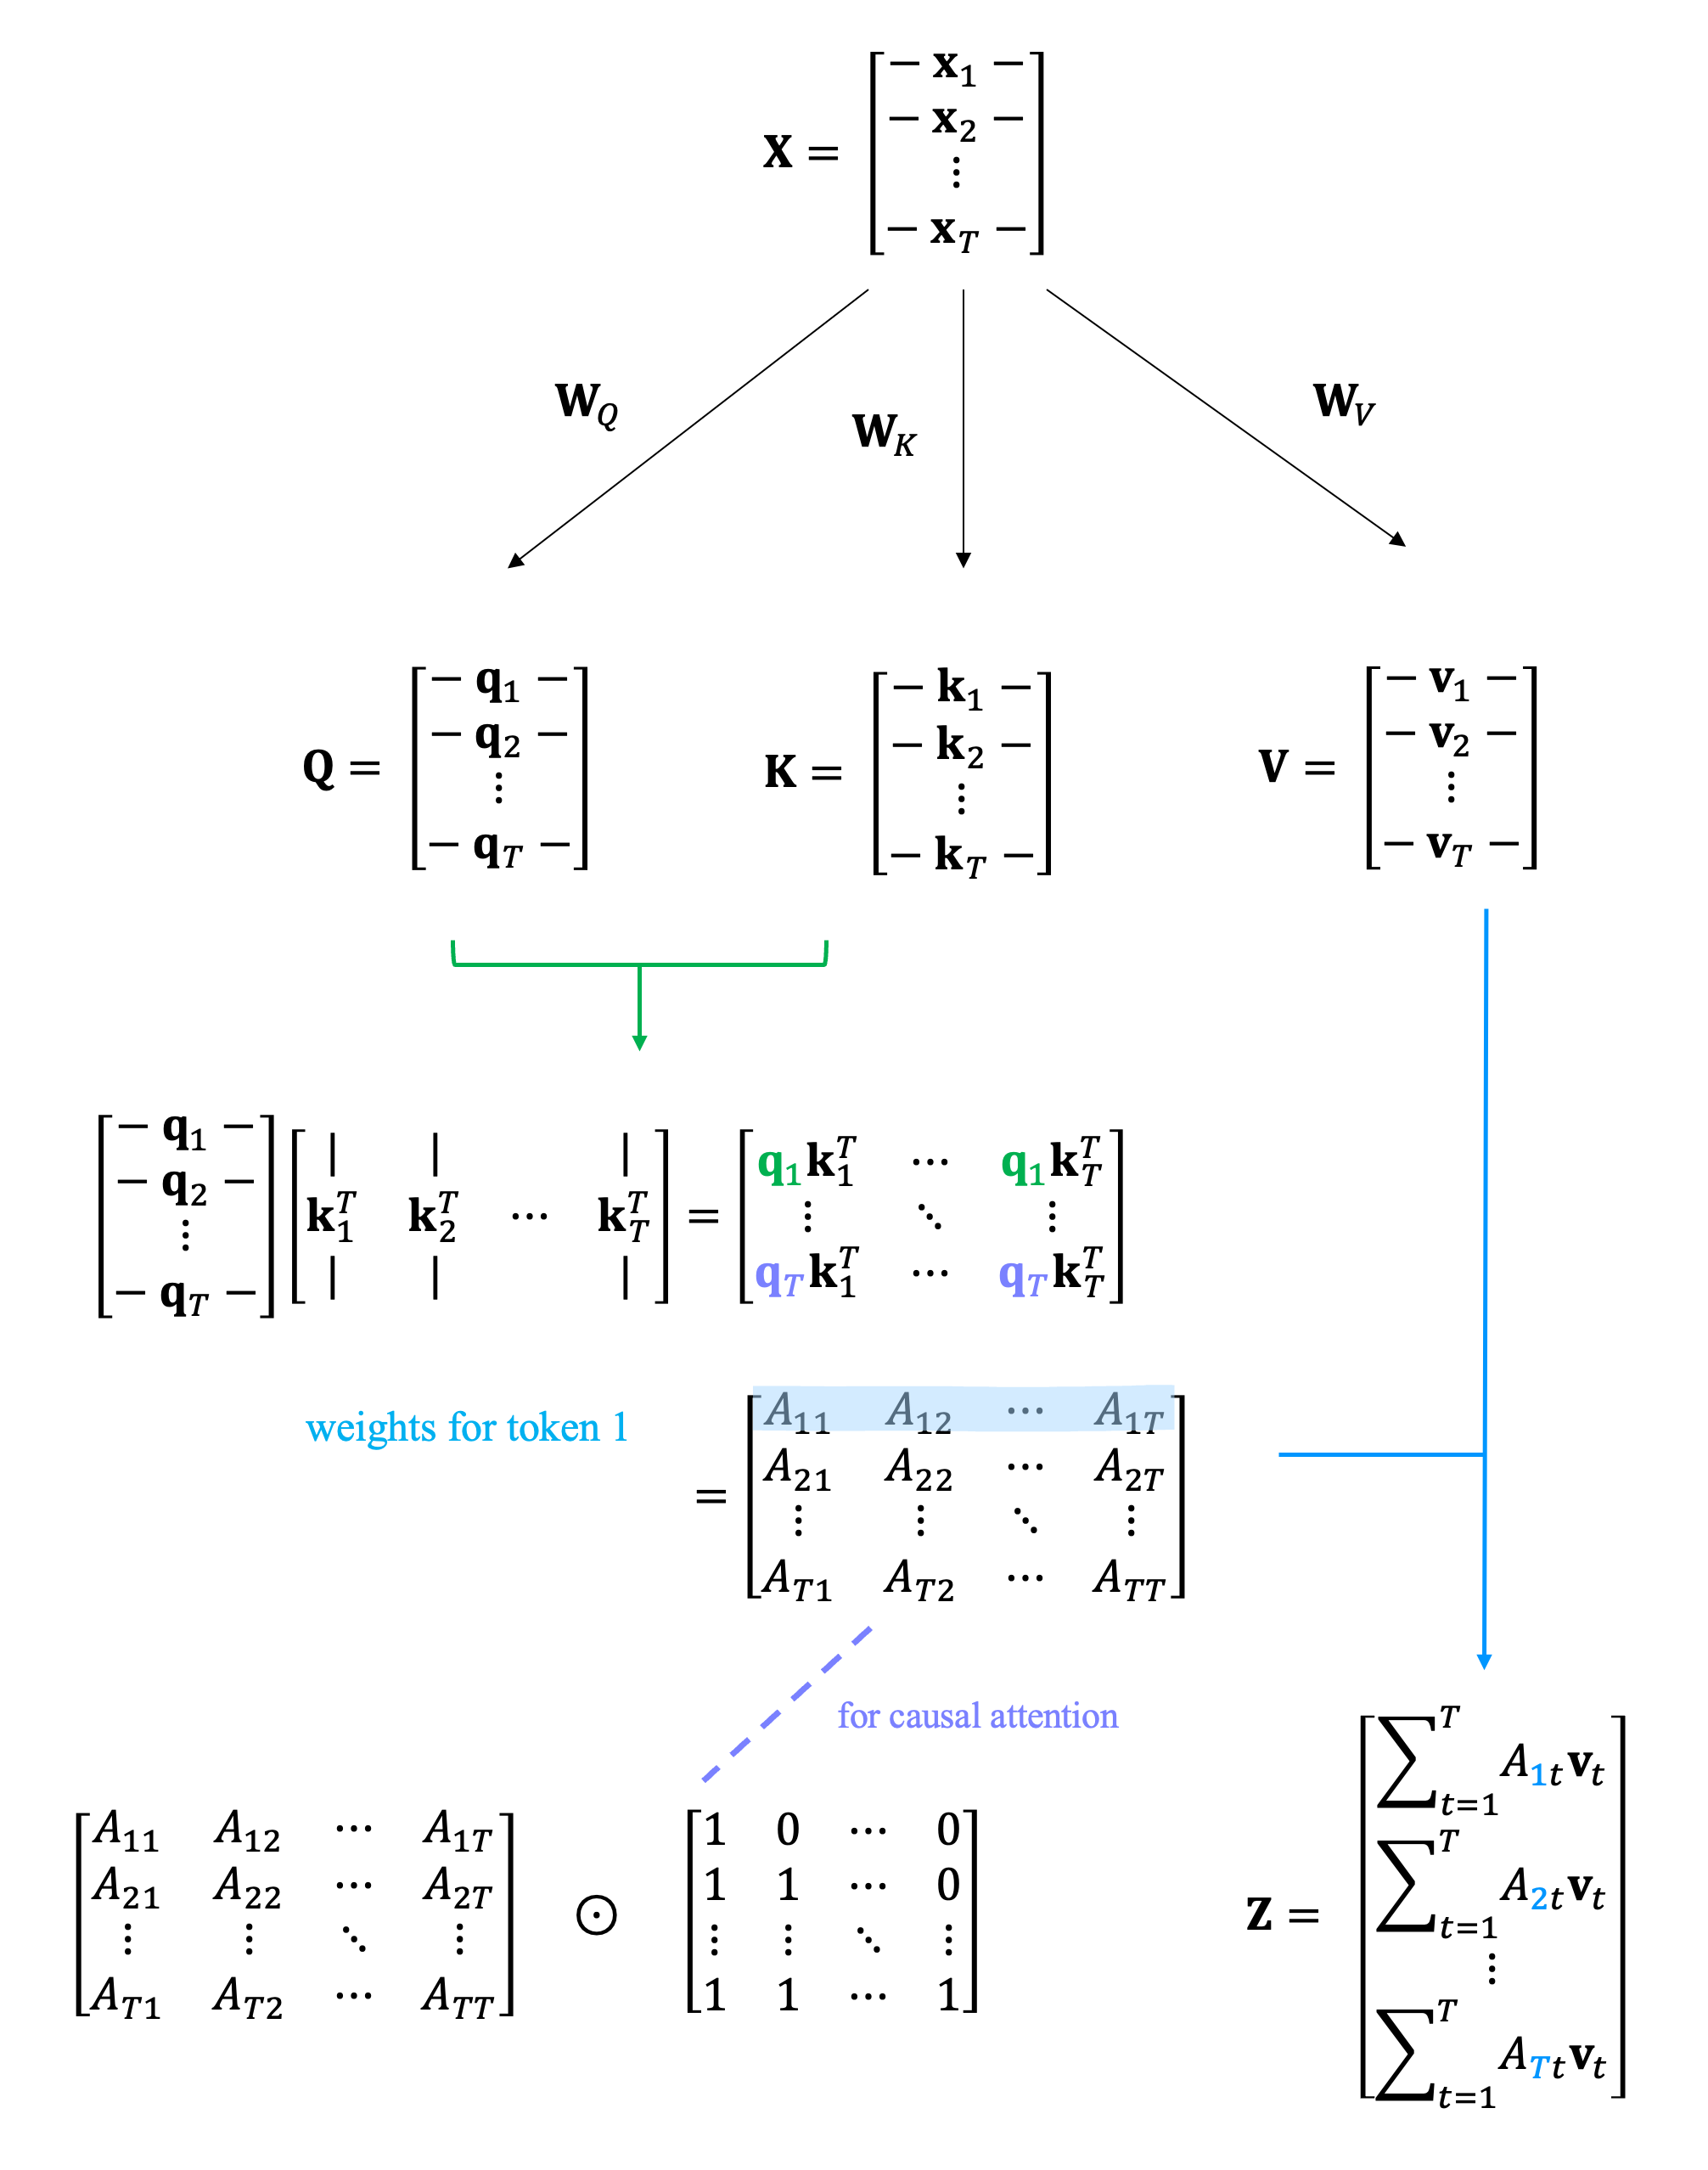
\includegraphics[scale=0.35]{imgs/self-attention.png}
\end{figure}

\clearpage
\subsection{Multi-Head Attention}
In multi-head attention, input $\bX$ is first passed through $H$ self-attention layer in parallel.
Then, the output from each head is concatenated together and fused by a linear projection
\[
\left[\textcolor{myblue}{\bZ^{(1)}}, \bZ^{(2)}, \ldots,  \bZ^{(H)}\right] \bW^O &= 
\begin{bmatrix}
\textcolor{myblue}{\bz_1^{(1)}} &  \bz_1^{(2)} & \ldots & \bz_1^{(H)} \\[0.8em]
\textcolor{myblue}{\bz_2^{(1)}} & \bz_2^{(2)} & \ldots & \bz_2^{(H)} \\[0.8em]
\vdots & \vdots & \ldots & \vdots \\[0.8em]
\textcolor{myblue}{\bz_T^{(1)}} & \bz_T^{(2)} & \ldots & \bz_T^{(H)}
\end{bmatrix}\bW^O
\] 

\begin{figure}[h]
\centering
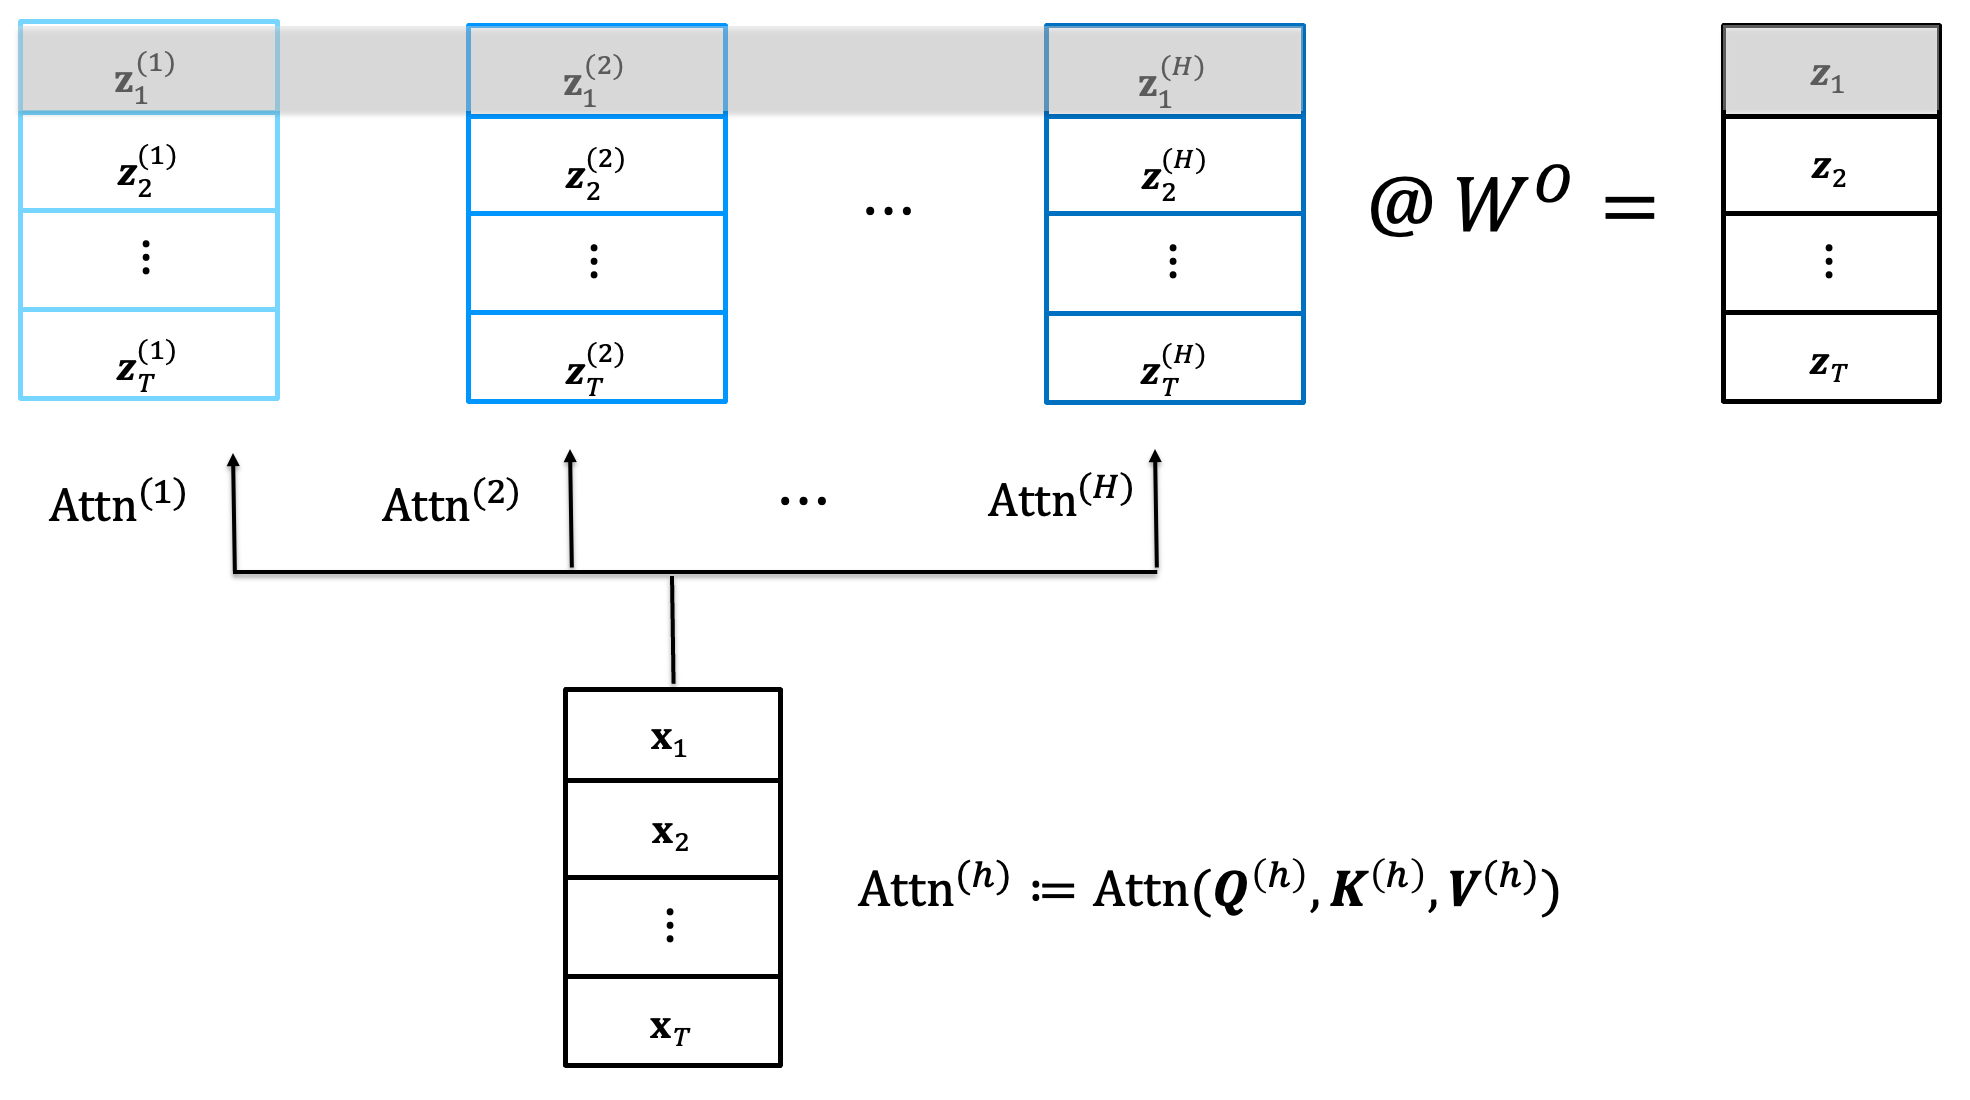
\includegraphics[scale=0.4]{imgs/multi-head.png}
\end{figure}

\clearpage
\subsection{KV-Cache}
During inference we still use causal masking because this is how the model being trained.
Let's look at a simple case where we only give the model a start token <s> and asks it to generate stuff:
\begin{figure}[!h]
\centering
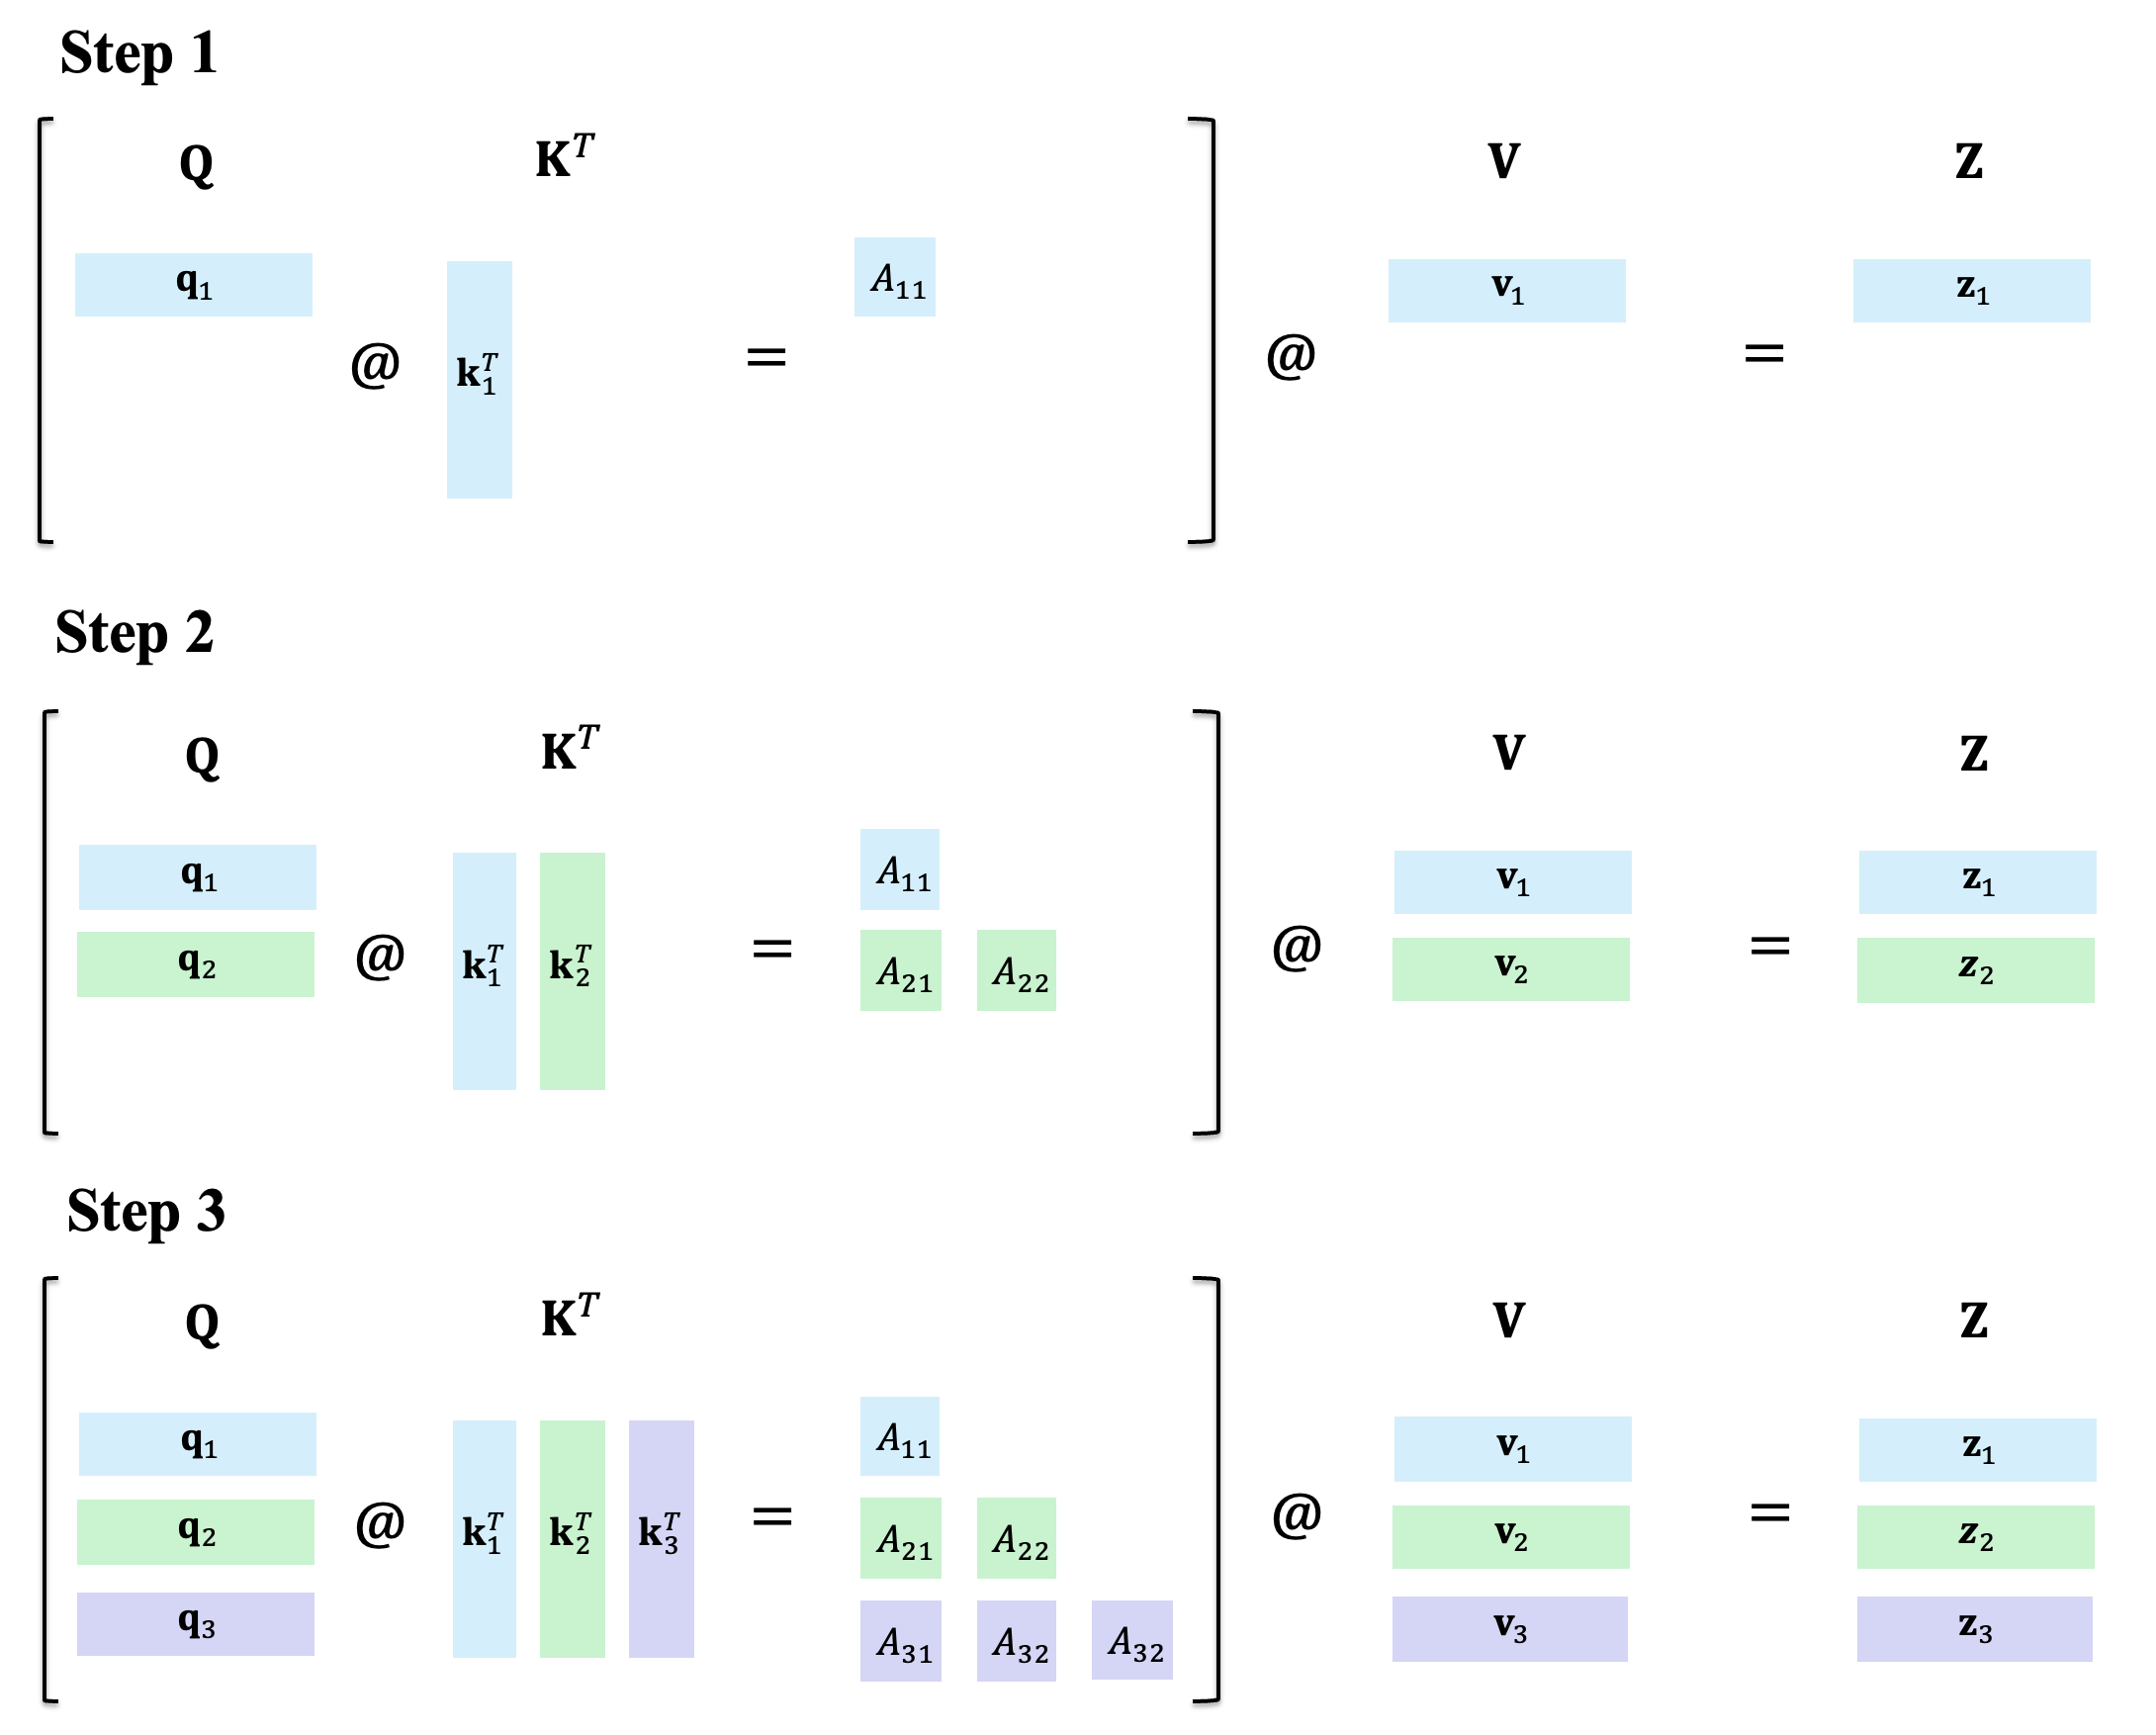
\includegraphics[scale=0.28]{imgs/no-cache.png}
\end{figure}

KV-cache is built on this two observations:
\begin{itemize}
	\item At each time step $t$, due to causal masking $\bk_{<t}$ and $\bv_{<t}$ will remain the same
	\item To predict <$\text{token}_{t+1}$> we only need embedding of <$\text{token}_{t}$>.
\end{itemize}
Therefore, we can make prediction efficiently by drop redundant and unnecessary computation
\begin{figure}[!h]
\centering
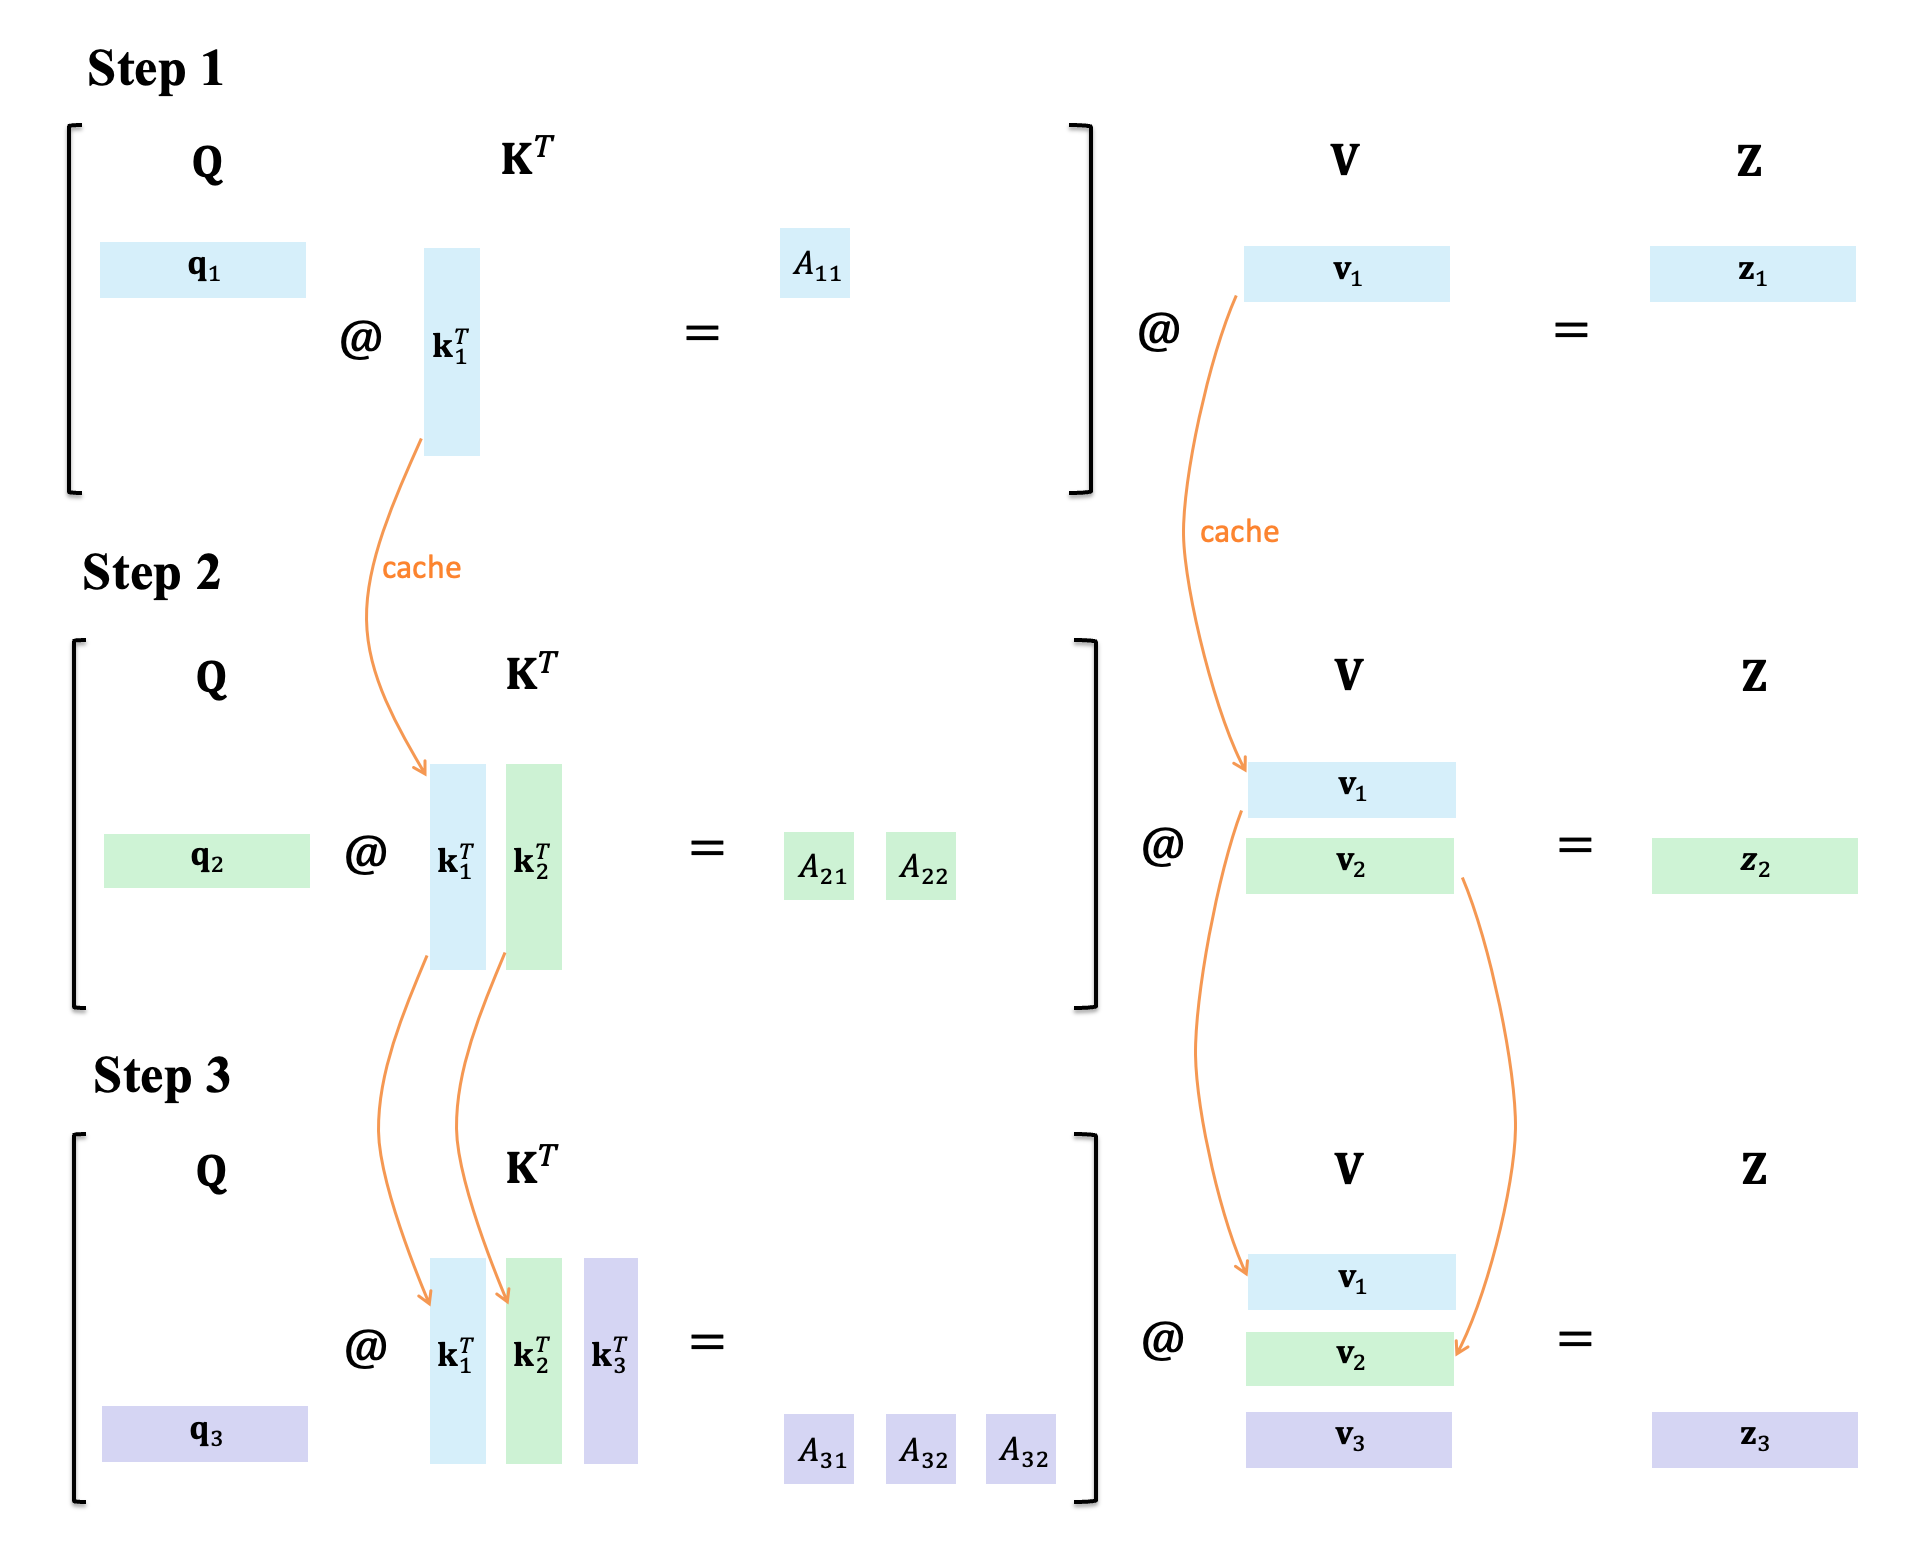
\includegraphics[scale=0.28]{imgs/cache.png}
\end{figure}


Basically we have

Token 1: [K1, V1] $\rightarrow$ Cache: [K1, V1]

Token 2: [K2, V2] $\rightarrow$ Cache: [K1, K2], [V1, V2]

...

Token n: [Kn, Vn] $\rightarrow$ Cache: [K1, K2, ..., Kn], [V1, V2, ..., Vn]


\clearpage
\section{Positional Embedding}

% print bibliography
\clearpage
\bibliography{bibliography} 

% Fill out appendix:
\newpage
\appendix

\end{document}
